\chapter{Wi-Fi-Konfiguration}
Wi-Fi ist im normalen Betrieb ausgeschaltet. Das Telefon während der Einrichtung etwa 10–20 cm von der Anzeige entfernt halten. Die Standard-Zugangsdaten lauten: Passwort 1234567890, Bedienoberfläche http://192.168.4.1.

USB trennen, Zündung beziehungsweise Stromversorgung einschalten und sofort den rückseitigen Taster drücken. Ein QR-Code erscheint. Mobile Daten am Telefon ausschalten, den QR-Code scannen und das Telefon mit dem Wi-Fi-Netz der Anzeige verbinden. Die Bedienoberfläche im Browser öffnen, Anwendung und passenden Sensor auswählen, speichern und die Zündung aus- und wieder einschalten.

Bei Verbindungsproblemen näher herangehen und prüfen, ob das Telefon trotz fehlendem Internet im Netz der Anzeige bleibt. Den Start mit QR-Code gegebenenfalls wiederholen. Der rückseitige Taster dient auch zur App-Bedienung und zur Auswahl des Bootmodus beim ersten Flashen.

USB ist für das erste Flashen vorgesehen; spätere Firmware-Updates über die Weboberfläche werden empfohlen. Vor USB-Nutzung alle Fahrzeugleitungen trennen. Die Anleitung der konkreten Firmware beachten; die Vorlage beschreibt weder ein Wiederherstellungsverfahren noch ein Upload-Menü.

\begin{figure}[H]
\centering
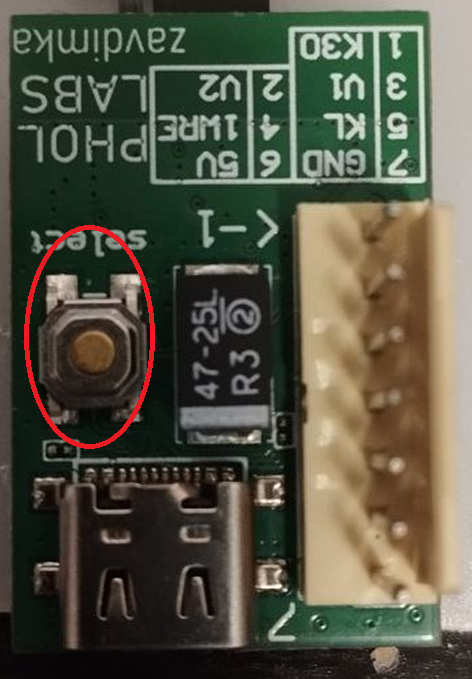
\includegraphics[width=.85\textwidth,height=.60\textheight,keepaspectratio]{figures/ivevo/image11.png}
\caption{Wi-Fi-Konfiguration}
\end{figure}
